\section{Hardware}\label{5_1_systemSetup}
\subsection{Components}\label{5_1_hardwareComponents}
%- System architecture of system --> Unity3D, Kinect SDK, Kinectstudio, VGB --> kinect sdk free to use since version X
In the following several hardware components of the system architecture will be described. Each component is important for the functionality of the SLS and the study afterwards. An overview can be seen in Figure~\ref{fig:5_3_systemArchitecture}.
% Kinect, Beamer, Screen, Slackline --> Alpidex High Performance

Since the focus of this thesis lies mainly on beginners the mobile slackline device \textit{alpidex POWER-WAVE 2.0}\footnote{\url{http://www.alpidex.com/fitness/slacklines/slackline-gestell-in-2-laengen-power-wave-2-0-inklusive-slackline/a-10288/}} is used.
It provides the needed mobility and independency due to its comparatively short length of three meters.
A major advantage is the possibility to set it up indoors as well as moving it in different positions with minimum effort.
The included slackline is tensed around brackets at both ends of the device.
%The middle rail is divided into two parts and needs to be put together.
It is placed in front of the \textit{Microsoft Kinect v2}, which is used as tracking device, like discussed in section~\textit{\nameref{trackingTechnologie}}. The Kinect itself is attached on a tripod with a height of about 90 cm.
A \textit{STEAM® MACHINE by ZOTAC}~\footnote{Technical details of the STEAM® MACHINE: Intel Core i5-6400T @ 2.2 GHz, NVIDIA GeForce® GTX 960, 8 GB RAM} served as development PC that fulfilled the recommended specs of the Kinect: \textit{Windows 8, 4 GB Memory, Physical dual-core processor with 3.1 GHz or faster, USB 3.0 Gen-2 controller, DirectX 11 Graphics card}. As visual output device a projector with a resolution of 1920x1080 was attached on a traverse system.
The interface was visualized on a projector screen with a size of 2,40 x 3,00 m to give the user a more immersive feeling.

\begin{figure}[htb]
	\centering
	\begin{minipage}[t]{1\linewidth}
		\centering
		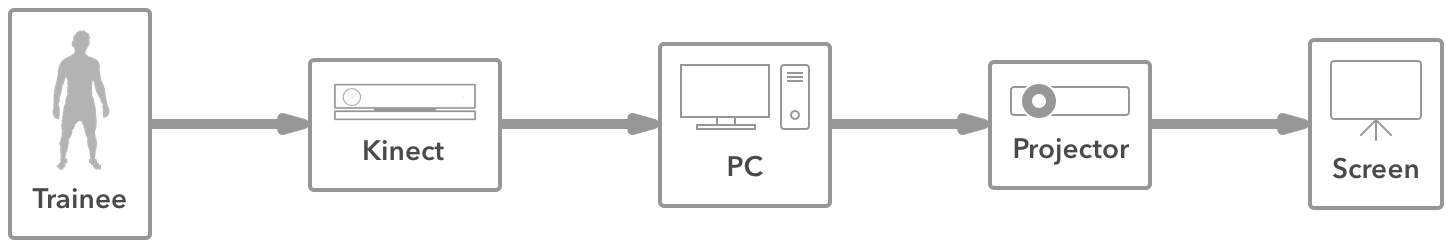
\includegraphics[width=1\linewidth]{Pictures/5_3_systemArchitecture}
		\caption{System overview}
		\label{fig:5_3_systemArchitecture}
	\end{minipage}
\end{figure}

\begin{comment}
\begin{figure}[htb]
	\centering
	\begin{minipage}[t]{1\linewidth}
		\centering
		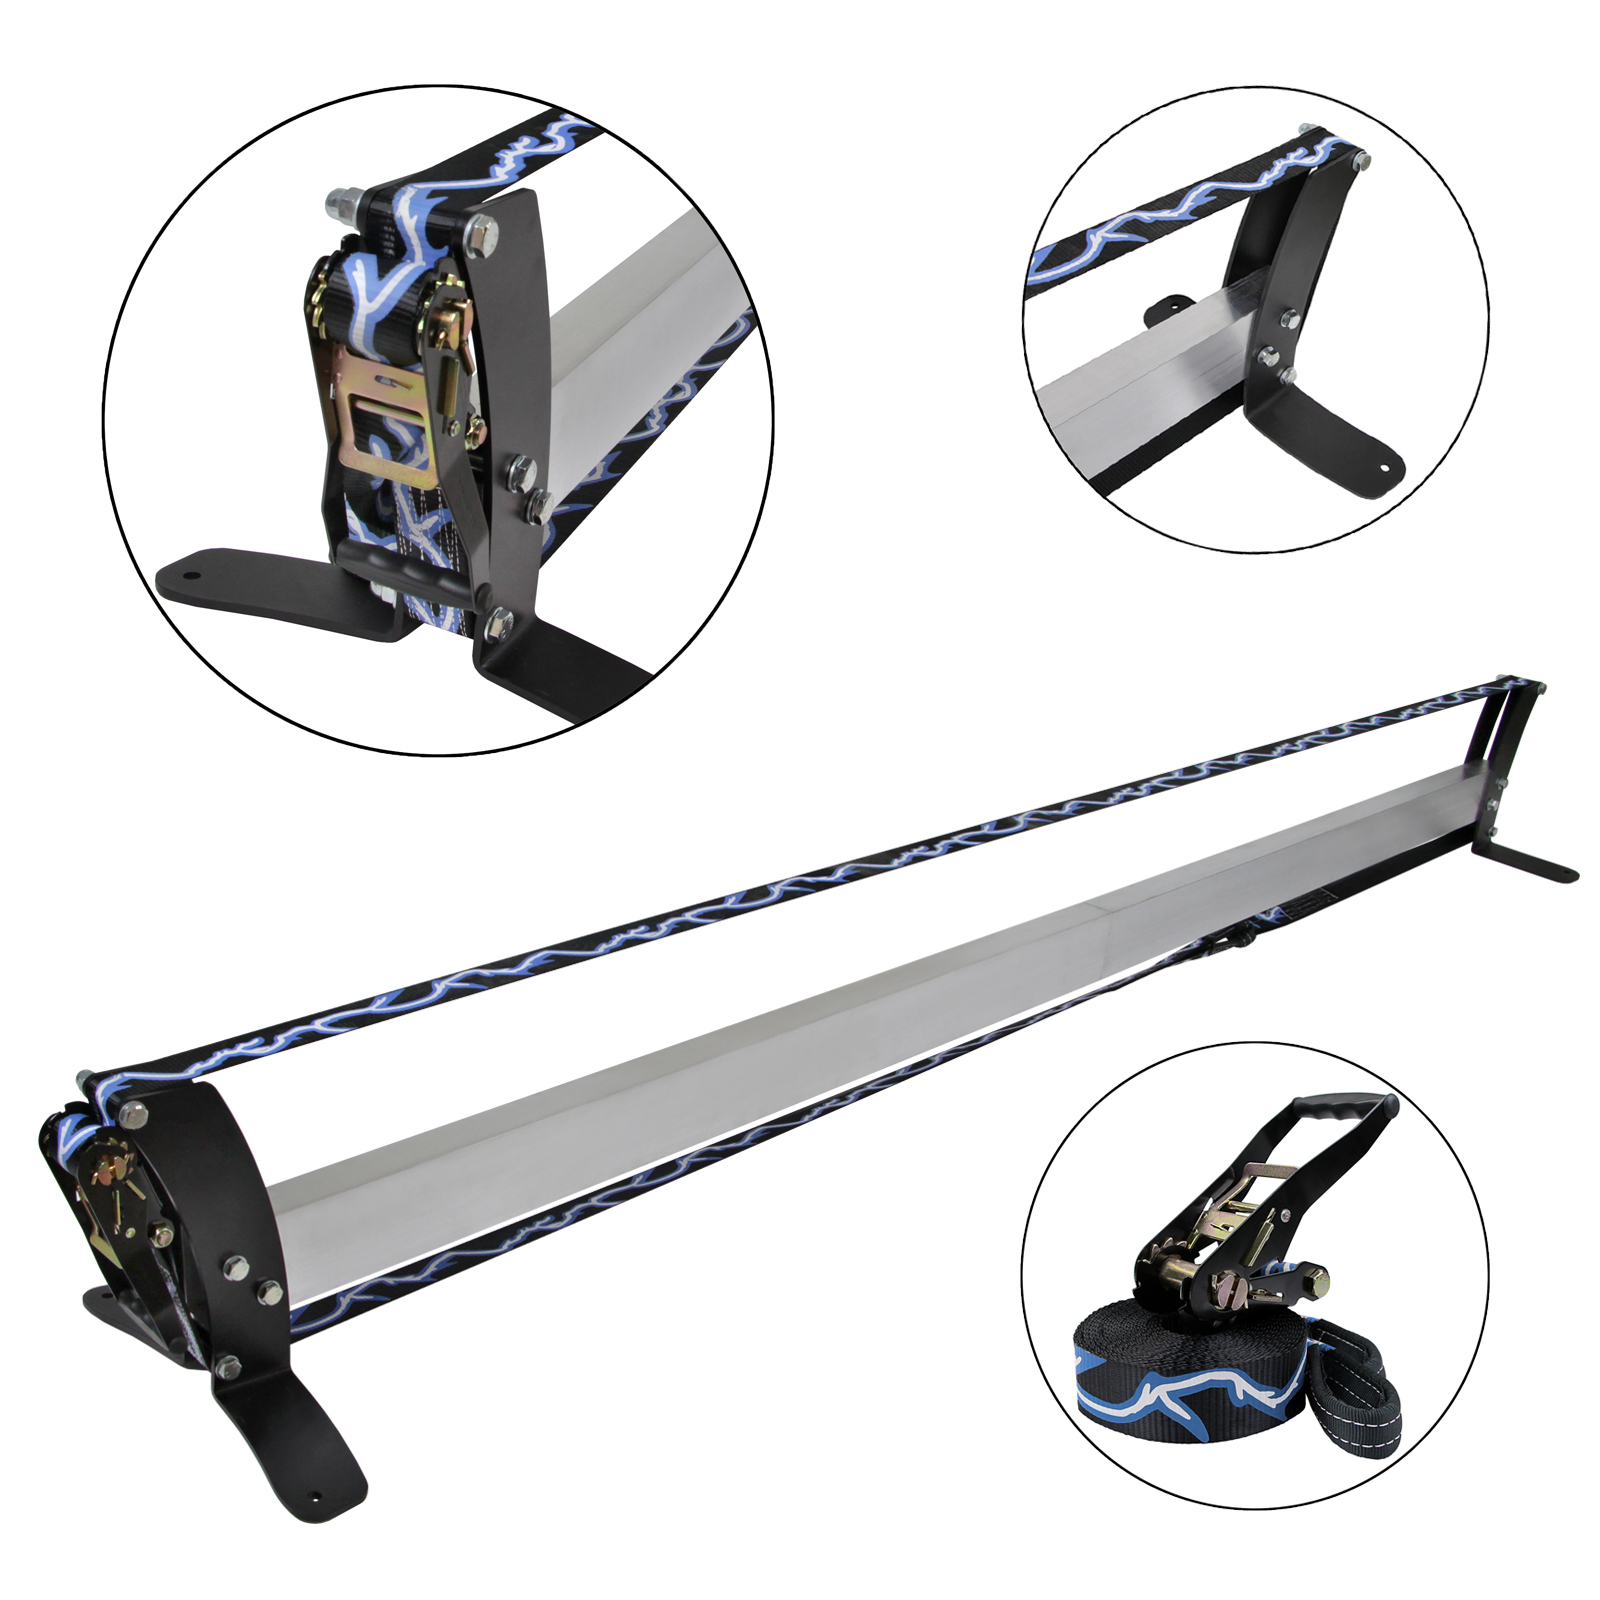
\includegraphics[width=0.44\linewidth]{Pictures/3_2_mobileSlackline}
		\caption{Mobile slackline \textit{alpidex POWER-WAVE 2.0}~\cite{alpidex2017-ms}}
		\label{fig:3_2_mobileSlackline}
	\end{minipage}
\end{figure}
\end{comment}

\subsection{Kinect and Slackline positioning}\label{5_1_technicalFeasibility}
Tracking a person on a slackline with the Kinect is very different from a common situation.
The combination of the slackline range, vibration of the line, and unpredictable movements because of balancing actions of the user could lead to imprecise and inaccurate input data for tracking.
%disturb the tracking performance.
%Furthermore, no comparable work exist about how to track user appropriately on a slackine with the Kinect.
The major approach is to compare different slackline positions (Vertical: 0 Degrees, Diagonal: 45 Degrees, Orthogonal: 90 Degrees) regarding multiple angles and heights of the Kinect (80 cm, 160 cm, 240 cm), which is attached on a tripod or traverse system.
This scenario clarifies how good a person can be tracked on the entire slackline as well as at the beginning of the line for study purposes of this thesis.
%Moreover, which is the best combination of the slackline and Kinect positioning to track a user on the entire line as well as for study purposes of this thesis.
%The testing person was recorded via \textit{KinectStudio}~\footnote{\url{https://developer.microsoft.com/de-de/windows/kinect/tools}}, a tool for recording clips out of the streaming data of the Kinect.

\subsubsection{Limitations of the Kinect} 
A considerable role plays the angle and tracking range of the Kinects' depth sensor in the positioning. Its angle of vision covers in horizontal 70 degrees and in vertical 60 degrees (Figure~\ref{fig:5_1_1_visionAngle}). Since the slackline is about 30 cm off the ground body parts of the user could be cropped depending on the Kinects' height and its angle. The total tracking range of the sensor covers a range between 0.5 and 4.5 meters, whereas the sweet spot area lies between 1 up to 4 meters (Figure~\ref{fig:5_1_1_trackingRange})~\cite{MicrosoftHIG2014-mh}. The mobile slackline device used in this thesis has a length of three meters and fits theoretically entirely within the sweet spot.
%it could lead to tracking problems by 
\begin{figure}[htb]
	\centering
	\begin{minipage}[t]{0.44\linewidth}
		\centering
		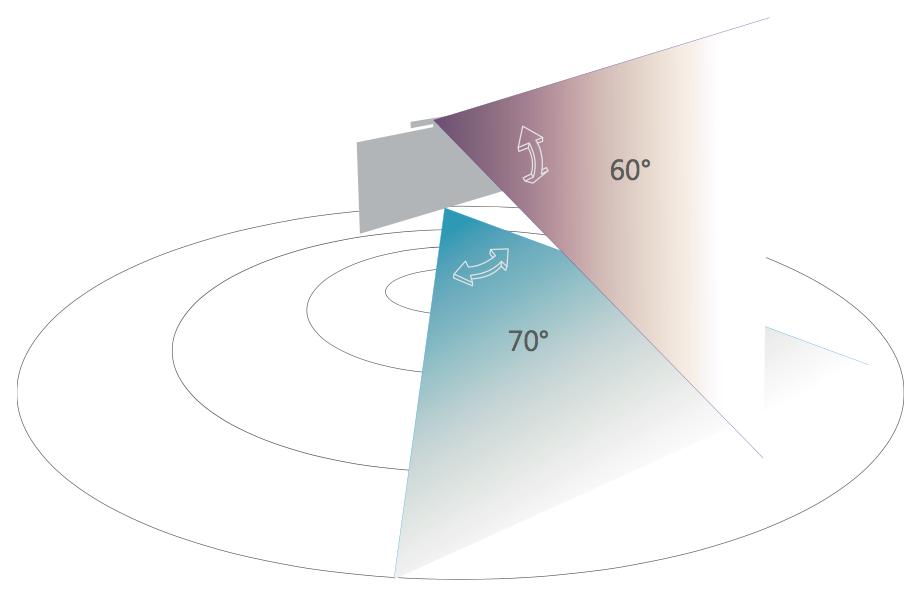
\includegraphics[width=1\linewidth]{Pictures/5_1_1_visionAngle}
		\subcaption{Angle of vision}
		\label{fig:5_1_1_visionAngle}
	\end{minipage}
	\hfill
	\begin{minipage}[t]{0.44\linewidth}
		\centering
		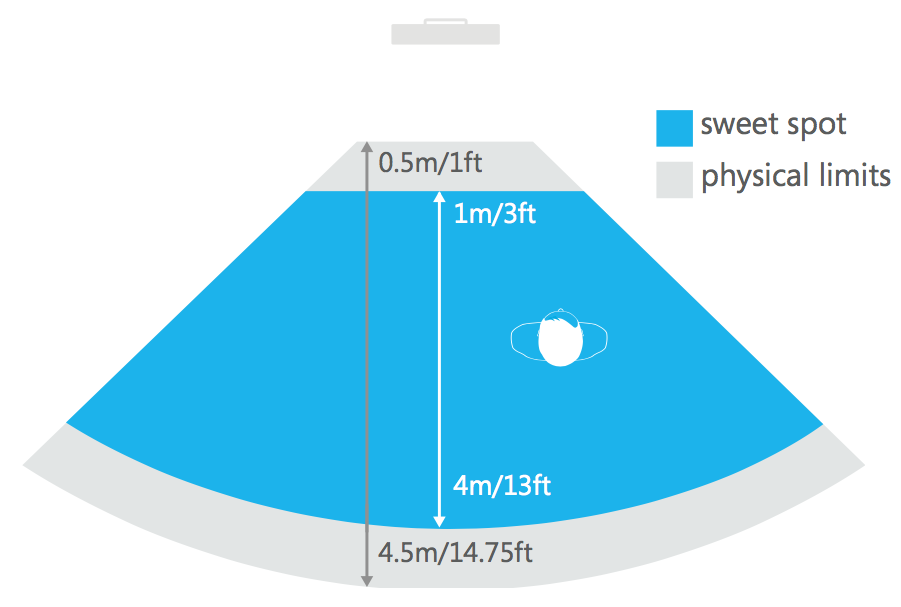
\includegraphics[width=1\linewidth]{Pictures/5_1_1_trackingRange}
		\subcaption{Kinect tracking range}
		\label{fig:5_1_1_trackingRange}
	\end{minipage}
	\caption{Limitations of the Kinect v2 sensor~\cite{MicrosoftHIG2014-mh}}
	\label{fig:5_1_1_sensorConstraints}
\end{figure}

%\subsubsection{Testing scenario}

%The test took place in the laboratory of the research group in the \textit{german reasearch center for artificial intelligence}~\footnote{\url{https://www.dfki.de/web/kontakt/dfki-saarbruecken}}. A big advantage of this is the large space to place the slackline easily in different variations. 
%The slackline is placed in three positions to the Kinect: frontal (0 Degree), diagonal (45 Degree) and sideways (90 Degree) \textbf{\todo{(Figure X - 1)}}. Each of this positions is tested regarding three different height levels of the Kinect: 80 cm, 160 cm, and 240 cm. Therefore it was attached on a tripod or traverse system (\textbf{\todo{Figure X - 2}}). At the end nine different combinations are covered to track a user on a slackline, which gives a general overview of the Kinect height to the slackline. The testing person was recorded via \textit{KinectStudio}~\footnote{\url{https://developer.microsoft.com/de-de/windows/kinect/tools}}, a tool for recording clips out of the streaming data of the Kinect.
%In the following the results discuss the feasibility and appropriate tracking positions.

\subsubsection{Best positioning for study purposes}
\textbf{\textit{Slackline Positioning}}

With a slackline positioned orthogonal (90 Degrees) to the Kinect, no interference regarding the limit of the tracking range can happen because the whole body is in a constant line with the tracking area. However, permanent overlapping of body parts resulted in problems to detect body joints with an appropriate accuracy and precision (Figure~\ref{fig:5_3_slacklineSideways}).
When placing the slackline diagonal (45 Degrees) the body is more visible to the sensor and showed better results.
%to the Kinect several body parts will not overlap.
%the frontal and end point of the slackline now differ in the vertical axis, which is unproblematic  \textbf{\todo{(Table X and Figure X)}}. 
%This could even result in a better trackability in matter of the depth field range, since the distance in the front shrinked and is therefore closer to the Kinect depth view. 
Tracking failure still happen especially when regaining equilibrium on the line. Mainly the joints of the arms and legs interfere with other body joints (Figure~\ref{fig:5_3_slacklineDiagonal}).
In addition, every time the user wants to interact with the Kinect she has to turn towards it, which leads to a more complicated user experience.
%which makes it also unusable.
%This results in a relatively bad skeletal tracking and depending on the executed exercise it can lead to detection problems.
Positioning the slackline vertical to the Kinect avoids this. Furthermore, the sensors' view can see the full body and track joints without any occlusion.
Problems occurred at the starting position of the slackline since it uses the entire tracking range.
The user stands here at the outermost limit of this range, where the detection of the Kinect begins to get worse (Figure~\ref{fig:5_3_slacklineVertical}).
Because of this the slackline must be arranged, such that the starting position of the line lies within the sweet spot area.
%Because of this the slackline must be positioned close to the Kinect for study purposes.
%The starting position of the line is now within the sweet spot area of the Kinect tracking range.
%Three main height levels were used to show the main differences of the tracking behaviour from the Kinect. It is mounted on a tripod and covers the heights of 0.80, 1.60 and 2.40 meters off the ground.
\begin{figure}[htb]
	\centering
	\begin{minipage}[t]{0.32\linewidth}
		\centering
		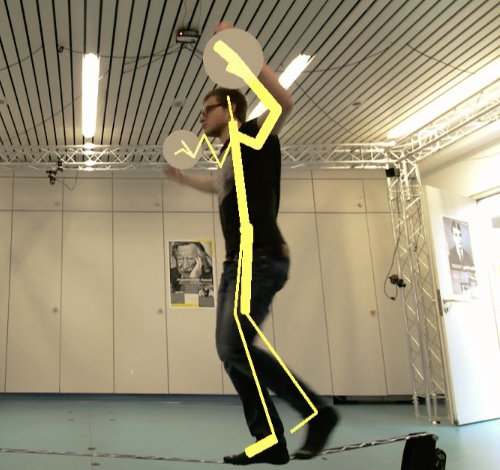
\includegraphics[width=1\linewidth]{Pictures/5_3_slacklineSideways}
		\subcaption{Sideways}
		\label{fig:5_3_slacklineSideways}
	\end{minipage}
	\hfill
	\begin{minipage}[t]{0.32\linewidth}
		\centering
		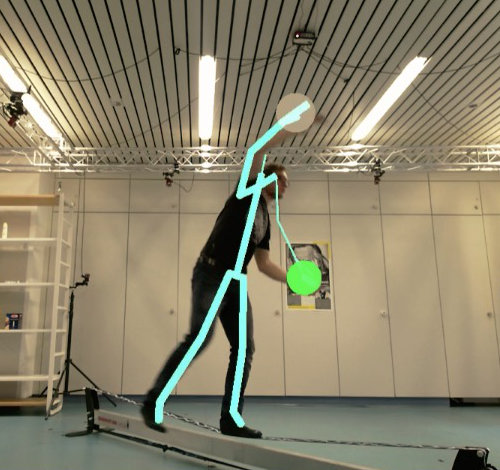
\includegraphics[width=1\linewidth]{Pictures/5_3_slacklineDiagonal}
		\subcaption{Diagonal}
		\label{fig:5_3_slacklineDiagonal}
	\end{minipage}
	\hfill
	\begin{minipage}[t]{0.32\linewidth}
		\centering
		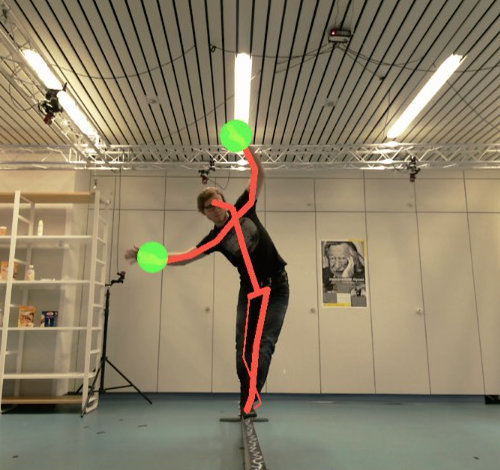
\includegraphics[width=1\linewidth]{Pictures/5_3_slacklineVertical}
		\subcaption{Vertical}
		\label{fig:5_3_slacklineVertical}
	\end{minipage}
	\caption{Different positions of the slackline. The coloured lines visualise the skeletal tracking of the Kinect. Thin lines represents inferred joints}
	\label{fig:5_3_slacklinePositionings}
\end{figure}

\textbf{\textit{Kinect Height}}

Beginning with a height of 2.40 meters the Kinect has a very steep view angle.
%to track the slackers' body on the full range of the slackline. 
Hereby, the tracking range shifts more downwards and shrinks in its height (Figure~\ref{fig:5_3_kinectHeightHigh}).
With users of a height above 1.85 m the starting position cannot be arranged for appropriate usage.
%If beginning at the starting position on the slackline the slacker reaches hereby immediately the end of the tracking area. 
The same problem applies for a Kinect height of 1.60 m. The view angle is more flat but the slackline must be positioned further away from the Kinect to prevent cropped body parts like the head or arms (Figure~\ref{fig:5_3_kinectHeightMiddle}).
%Also the further she walks towards the Kinect the more joints of the feet overlap.
%With a height between 1.60 and 1.20 meters the view angle is more flat but the slackline must be positioned further away from the Kinect to prevent cropped body parts like the head or arms (Figure\ref{fig:5_3_kinectHeightMiddle}).
A height of 1.20 up to 0.80 meters results in a flatter view angle and therefore in a more homogeneous view and tracking range (Figure~\ref{fig:5_3_kinectHeightLow}).
The body is fully visible in the entire tracking range and not limited in the height of the Kinect view.
Additionally the Kinect is in a position that won't disturb the visual sense slacker during her training on the slackline, e.g. by setting a focus point in front of her.
%Problems can occur with positioning the Kinect on a lower height. It can lead to cropped body parts like the head or arms at the very end of the slackline.

\begin{figure}[htb]
	\centering
	\begin{minipage}[t]{0.32\linewidth}
		\centering
		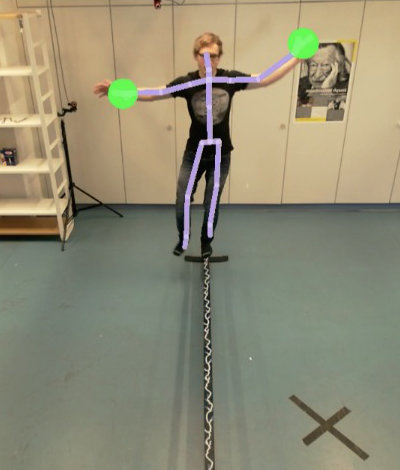
\includegraphics[width=1\linewidth]{Pictures/5_3_kinectHeightHigh}
		\subcaption{Kinect height of 2.40 m}
		\label{fig:5_3_kinectHeightHigh}
	\end{minipage}
	\hfill
	\begin{minipage}[t]{0.32\linewidth}
		\centering
		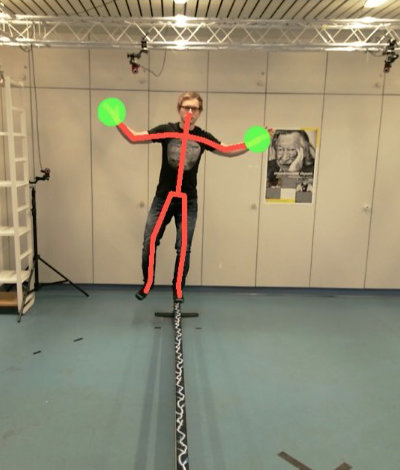
\includegraphics[width=1\linewidth]{Pictures/5_3_kinectHeightMiddle}
		\subcaption{Kinect height of 1.60 m}
		\label{fig:5_3_kinectHeightMiddle}
	\end{minipage}
	\hfill
	\begin{minipage}[t]{0.32\linewidth}
		\centering
		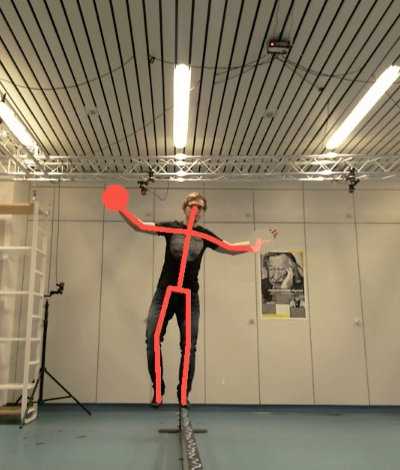
\includegraphics[width=1\linewidth]{Pictures/5_3_kinectHeightLow}
		\subcaption{Kinect height of 0.80 m}
		\label{fig:5_3_kinectHeightLow}
	\end{minipage}
	\caption{Kinect view on different heights. The coloured lines visualises skeletal tracking.}
	\label{fig:5_3_kinectHeights}
\end{figure}

%The tracking and view is more homogeneous and the angle flatter, which results in the possibility to use the full depth range. With a higher attachment the angle will be too steep, which results in less depth range, as well as more occlusions of body parts can occur.
\begin{comment}
\rowcolors{2}{tablerowgray}{tablerowgray}
\begin{table}[h!]
\centering
%\arrayrulecolor{white}
\renewcommand{\arraystretch}{1}
\begin{tabular}{| c c c | c c | c c c |}
\hline
\rowcolor{tableheadergray} & \multicolumn{7}{| c |}{\textbf{Slackline Positioning (m)}} \\ 
\rowcolor{tableheadergray} \textbf{Kinect Height (m)} & \multicolumn{2}{ c |}{\textbf{Vertical}} & \multicolumn{2}{| c |}{\textbf{Diagonal}} & \multicolumn{3}{ c |}{\textbf{Sideways}}\\
\rowcolor{tableheadergray} & \textbf{Front} & \textbf{Back} & \textbf{Front} & \textbf{Back} & \textbf{Front} & \textbf{Back} & \textbf{Mid} \\
\hline
2,40 & 1.30 & 4.30 & 1.90 & 3.80 & 3.00 & 3.00 & 2.70 \\
\hline
1.60 & 1.70 & 4.70 & 2.10 & 4.00 & 3.00 & 3.00 & 2.70 \\
\hline
0.80 & 1.30 & 4.30 & 1.90 & 3.80 & 2.60 & 2.60 & 2.10 \\
\hline
\rowcolor{green} 0.80 - 1.20 & 0.00 & 4.00 & - & - & - & - & - \\
\hline
\end{tabular}
\caption{Combination of Kinect height and slackline positioning}
\label{table:1}
\end{table}
\end{comment}

% But since beginner will use the entire slackline range it can be neglected.
The best combination resulted in placing the slackline vertical and having a Kinect height of 0.80 up to 1.20 meters. Hereby, the Kinect can track the entire body with nearly no joint overlap.
Since the focus of the study in this thesis lies mainly on beginners, the starting position of the slackline is important and must not lie at the outermost tracking range.
Hence, it makes more sense to move the slackline very close to the Kinect. The starting position on the line fits then within the sweet spot area.
%a higher tracking confidence is possible.
%plays an important role and 
%because the very end of the line is not necessary for the study.
%a little bit of slackline is cropped out of the view but 
%A higher tracking confidence is possible at the starting position, which is more important in this case \textbf{\todo{(Figure X)}}.
%This results in a relatively bad skeletal tracking and depending on the executed exercise it can lead to detection problems.